% !TeX spellcheck = en_GB
\documentclass[AERbeamer%              style
              ,optEnglish%            language
              %,handout%               deactivate animation
              ,optBiber%               bibliography tool
              ,optBibstyleAlphabetic%
              ,optBeamerClassicFormat% 4:3 format
              %,optBeamerWideFormat%   16:9 format
              ]{AERlatex}%
\setbeameroption{show notes}% Show all notes
%
% Set paths
\graphicspath{{figures_lecture_1/}}%
\addbibresource{literature.bib}%
%
% Package Imports
%\usepackage{media9}
\usepackage{graphicx}
\usepackage{multimedia}
\usepackage{subcaption}
\usepackage{amsmath}
%
% set meta data
\title{Probabilistic Programming for Scientific Discovery}%
\subtitle{Lecture 1}
\author{Ludger Paehler}% (optional)
\date{\AERutilsDate{29}{7}{2020}}% (optional)
\institute{Lviv Data Science Summer School}% (optional)
%
% Setup of header and footer
\AERbeamerSetupHeader{\AERlayoutHeaderCDChair}%
\AERbeamerSetupFooterCD%
%\AERbeamerSetupFooterSlideNumberOnly%
%
\begin{document}%
%
% Start with titlepage
\AERbeamerTitlePageDefault%
%
%\begin{frame}{Title of Slide}{Subtitle of Slide}%
%    \blindtext%
%\end{frame}%
%

% Slide 0: Table of Contents
\begin{frame}{Table of Contents}{}%
    % Contents
    \tableofcontents
\end{frame}%


% Course outline
\section{Course Outline}

\begin{frame}[c]{Course Outline}
    \centering
    \begin{itemize}
        \item 4 Lectures
        \begin{enumerate}
            \item Foundational Knowledge
            \item Inference Engines \& Introduction to Turing.jl
            \item Hierarchical Bayesian Approaches \& Bayesian Deep Learning
            \item The Connection to Scientific Problems
        \end{enumerate}
        \item 3 Tutorials for Self-Paced Consumption
        \begin{enumerate}
            \item In-Depth Introduction to Probabilistic Programming Systems with Turing.jl
            \item Bayesian Approaches in Probabilistic Programming
            \begin{itemize}
                \item Bayesian Deep Learning
                \item Hierarchical Bayesian Modelling
            \end{itemize}
            \item Machine-Learning Based Design with Probabilistic Programming
        \end{enumerate}
    \end{itemize}
\end{frame}


% Etalumis and DreamCoder references to be inserted here! -- as footnotes quite probably.
\begin{frame}[c]{Lecture 1}
    \centering
    \begin{itemize}
        \item Example Applications of Probabilistic Programming
        \begin{enumerate}
            \item \textit{ETALUMIS: Bringing Probabilistic Programming to Scientific Simulators at Scale}
            \item \textit{DreamCoder: Growing Generalizable, Interpretable Knowledge with Wake-Sleep Bayesian Program Learning}
        \end{enumerate}
        \item Why do we even need Probabilistic Programming?
        \item Underlying Theoretical Ideas
        \item Different Types of Probabilistic Programming Systems
    \end{itemize}
\end{frame}


% Turing reference to be inserted here!
\begin{frame}[c]{Lecture 2}
    \centering
    \begin{itemize}
        \item Approaches to Inference - the Inference Engine
        \item Practical Introduction to a Probabilistic Programming Framework
        \item Extending our learned ideas to a more complex example
    \end{itemize}
\end{frame}


% References need to be inserted here!
\begin{frame}[c]{Lecture 3}
    \centering
    \begin{itemize}
        \item Bayesian Hierarchical Approaches
        \item Bayesian Deep Learning, including but not limited to
        \begin{itemize}
            \item Inference Networks
            \item Uncertainty Quantification
        \end{itemize}
        \item Marrying Deep Learning Frameworks with Probabilistic Programming for Type 2 Machine Learning
    \end{itemize}
\end{frame}


\begin{frame}[c]{Lecture 4}
    \centering
    \begin{itemize}
        \item Interaction with Scientific Simulators
        \begin{itemize}
            \item What types of simulators would I want to link to?
            \item What are the hidden pitfalls?
        \end{itemize}
        \item Areas of application
        \begin{itemize}
            \item Robotics
            \item Physics
            \item Engineering
            \item Machine-Learning Based Design
        \end{itemize}
        \item Extensive Machine-Learning Based Design Example
    \end{itemize}
\end{frame}



% Examples, examples, examples
\section{Example Applications of Probabilistic Programming}


% Example 1 (~10 slides?)
\subsection{ETALUMIS: Bringing Probabilistic Programming to Scientific Simulators at Scale}

\begin{frame}[c]{ETALUMIS}{Bringing Probabilistic Programming to Scientific Simulators at Scale}
    \centering
    \begin{itemize}
        \item Blub
    \end{itemize}
\end{frame}



% Example 2 (~10 slides?)
\subsection{DreamCoder: Growing Generalizable, Interpretable Knowledge with Wake-Sleep Bayesian Program Learning}

% DreamCoder Slide 1: Rough summary
\begin{frame}[c]{DreamCoder \footnote{Ellis, K., Wong, C., Nye, M., Sable-Meyer, M., Cary, L., Morales, L., Hewitt, L., Solar-Lezama, A. and Tenenbaum, J.B., 2020. DreamCoder: Growing generalizable, interpretable knowledge with wake-sleep Bayesian program learning. arXiv preprint arXiv:2006.08381.}}{Growing Generalizable, Interpretable Knowledge with Wake-Sleep Bayesian Program Learning}
    \centering
    \begin{itemize}
        \item Constructs domain-specific languages (DSLs) for scientific problems combined with a neural network,
              which embodies a learned domain-specific search strategy
        \begin{itemize}
            \item Learns both the system prior and the needed inference algorithm
        \end{itemize}
        \item Practically constructs a library of symbolic abstractions in a wake-sleep manner and applies said library
              to the solving of the chosen problem at hand
        \item Utilizes wake-sleep learning % reference needed here
        \begin{itemize}
            \item During \textit{sleep} the system consolidates its abstractions from the programs found during \textit{wake}
                  and improves upon the neural network recognition model by imagining new samples
            \item During \textit{wake} the generative model is exploited on the problem domain to find the programs with the
                  highest posterior probability
        \end{itemize}
    \end{itemize}
\end{frame}


% Slide 2: Knowledge-Hierarchy and Probabilistic Inference
\begin{frame}[c]{DreamCoder}
    \centering
    \begin{itemize}
        \item Knowledge is accumulated in a multilayered hierarchy with knowledge and skills being
              successively learned over time, i.e. the knowledge is bootstrapped from very simple
              examples to ever more complex cases
        \item Can be broken down to a probabilistic inference procedure, i.e. observing task $X$ and
              inferring program $\rho_{x}$ to solve task $x \in X$ combined with a prior distribution
              over program, which migh solve tasks in the domain
        \begin{align*}
            \rho_{x} &= \underset{\substack{\rho: \\ Q(\rho|x) \text{ is large}}}{\arg \max} P[\rho | x, L] \propto P[x | \rho ] P[\rho | L], \text{ for each task } x \in X &Wake \\
            L &= \underset{L}{\arg \max} P[L] \prod_{x \in X} \underset{\rho \text{ a refactoring of } \rho_{x}}{\max} P[x | \rho] P[\rho | L] &Sleep: Abstraction \\
            \text{Train } &Q(\rho | x) \approx P[\rho | x, L], \text{ where } x \sim X \text{ ('replay') or } x \sim L \text{ ('fantasy')} & Sleep: Dreaming
        \end{align*}
    \end{itemize}
\end{frame}


% DreamCoder Slide 3: Overall algorithm
\begin{frame}[c]{DreamCoder}
    \centering
    \begin{figure}
        \centering
        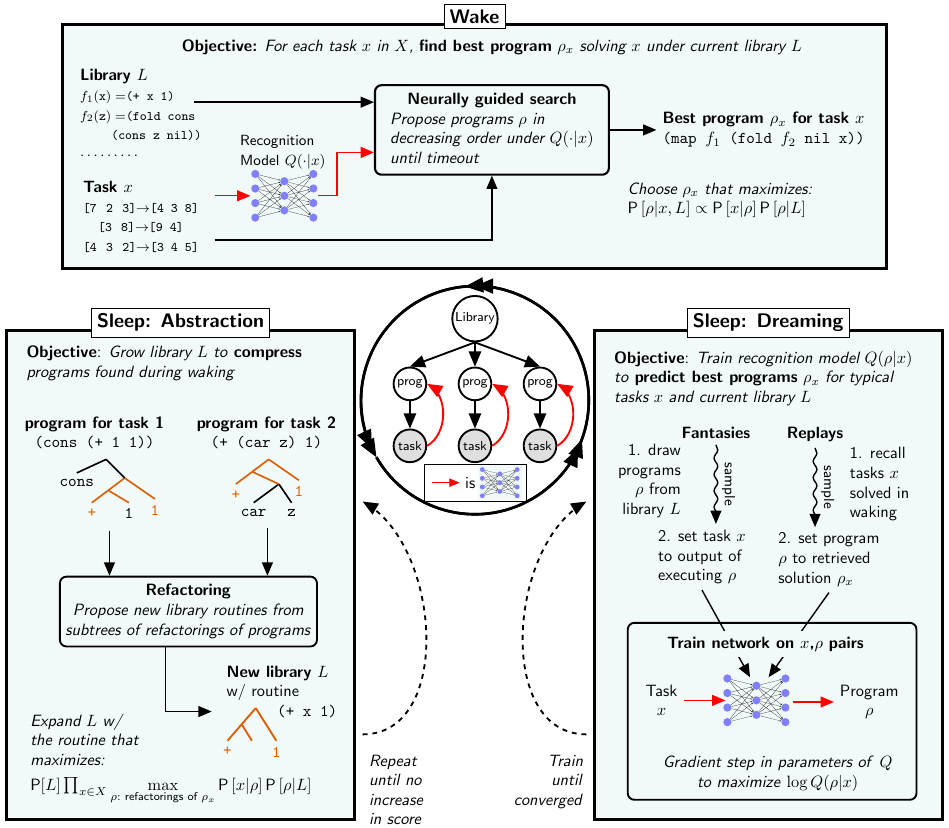
\includegraphics[width=0.5\textwidth]{DreamCoderAlgorithmCycle.png}
        \caption{Algorithm Cycle of DreamCoder}
    \end{figure}
\end{frame}


% DreamCoder Slide 4: Algorithm
\begin{frame}[c]{DreamCoder}
    \centering
    \begin{figure}
        \centering
        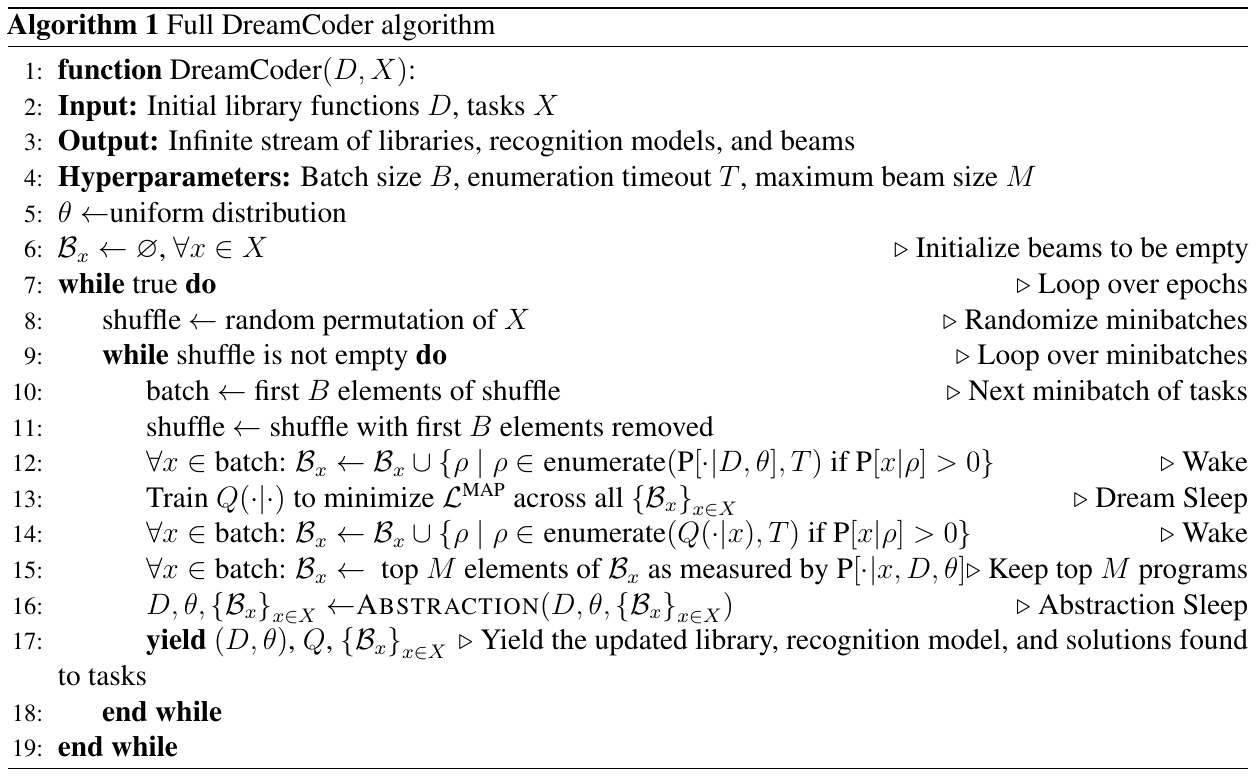
\includegraphics[width=0.7\textwidth]{DreamCoderAlgo.png}
    \end{figure}
\end{frame}


% DreamCoder Slide 5: Algorithm Structure
\begin{frame}[c]{DreamCoder}
    \centering
    \begin{figure}
        \centering
        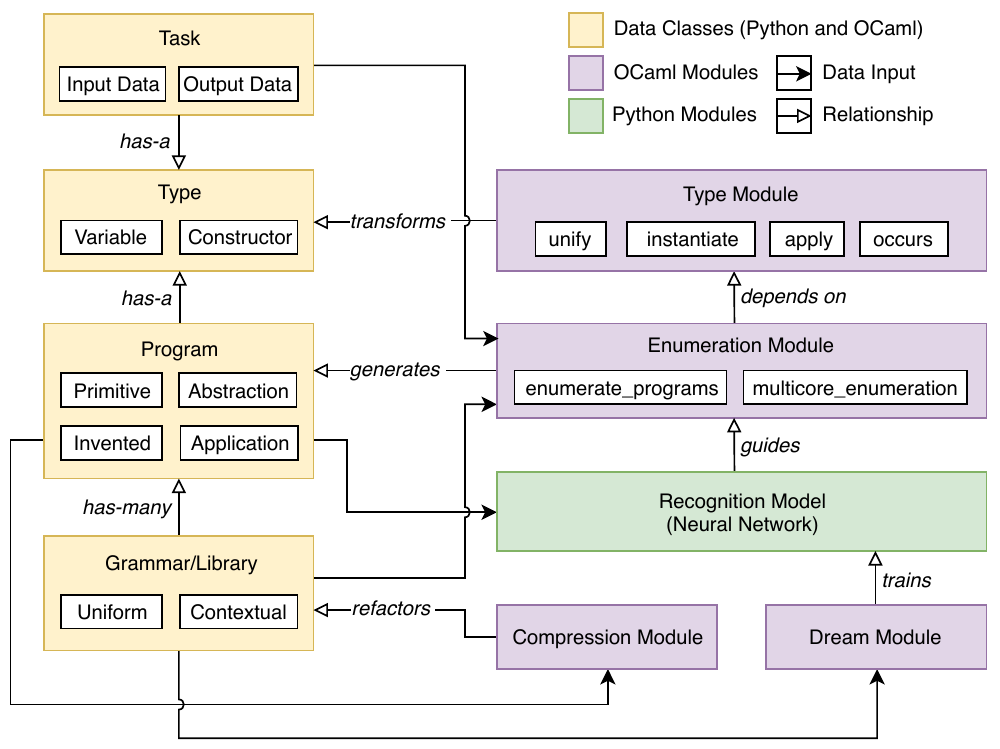
\includegraphics[width=0.6\textwidth]{DreamCoderDataClasses.png}
        \caption{Different data-classes in DreamCoder.}
    \end{figure}
\end{frame}


% DreamCoder Slide 6: Program Flowchart
\begin{frame}[c]{DreamCoder}
    \centering
    \begin{figure}
        \centering
        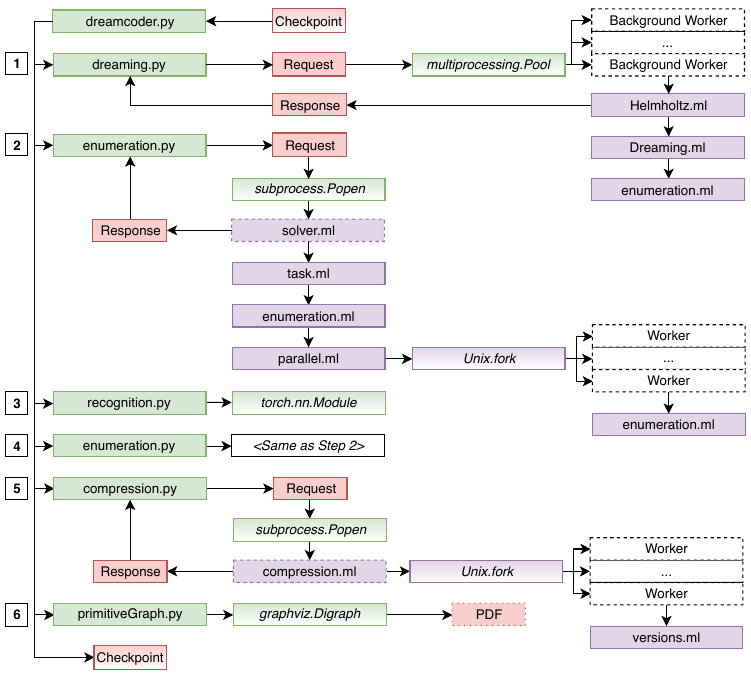
\includegraphics[width=0.5\textwidth]{DreamCoderProgramFlowchart.png}
        \caption{Program Flowchart: Phase 1, Dreaming. Phase 2, 1st Program Enumeration. Phase 3, Recognition Model Training.
                 Phase 4, 2nd Program Enumeration. Phase 5, Abstraction (Compression). Phase 6, Library Visualization.}
    \end{figure}
\end{frame}


% DreamCoder Slide 7: Helmholtz Machine Innuendo 1
\begin{frame}[c]{Recap: Helmholtz Machine \footnote{Graves, A., Wayne, G. and Danihelka, I., 2014. Neural turing machines. arXiv preprint arXiv:1410.5401.}
                                          \footnote{YouTube: DeepMind x UCL | Deep Learning Lectures | 8/12 | Attention and Memory in Deep Learning}}
    \centering
    \begin{itemize}
        \item Blub
    \end{itemize}
\end{frame}


% DreamCoder Slide 8: Helmholtz Machine Innuendo 2
\begin{frame}[c]{Recap: Helmholtz Machine}
    \centering
    \begin{itemize}
        \item Blub 2
    \end{itemize}
\end{frame}


% DreamCoder Slide 9: Helmholtz Machine Innuendo 3  <- Priority sort
\begin{frame}[c]{Recap: Helmholtz Machine}
    \centering
    \begin{itemize}
        \item Blub 3
    \end{itemize}
\end{frame}


% DreamCoder Slide 10: Differentiable Neural Computers (Outlook)
\begin{frame}[c]{Outlook: Differentiable Neural Computer \footnote{Graves, A., Wayne, G., Reynolds, M., Harley, T., Danihelka, I., Grabska-Barwińska, A., Colmenarejo,
                                                                   S.G., Grefenstette, E., Ramalho, T., Agapiou, J. and Badia, A.P., 2016. Hybrid computing using a
                                                                   neural network with dynamic external memory. Nature, 538(7626), pp.471-476.}}
    \centering
    \begin{itemize}
        \item Differentiable Neural Computer
    \end{itemize}
\end{frame}


% DreamCoder Slide 10: Compositional Nature
\begin{frame}[c]{DreamCoder}
    \centering
    \begin{itemize}
        \item Due to its compositional nature, representations of problems can be bootstrapped from earlier, simpler version of
              the scientific task to more and more complex settings
    \end{itemize}
    \vspace{1cm}
    \begin{figure}
        \centering
        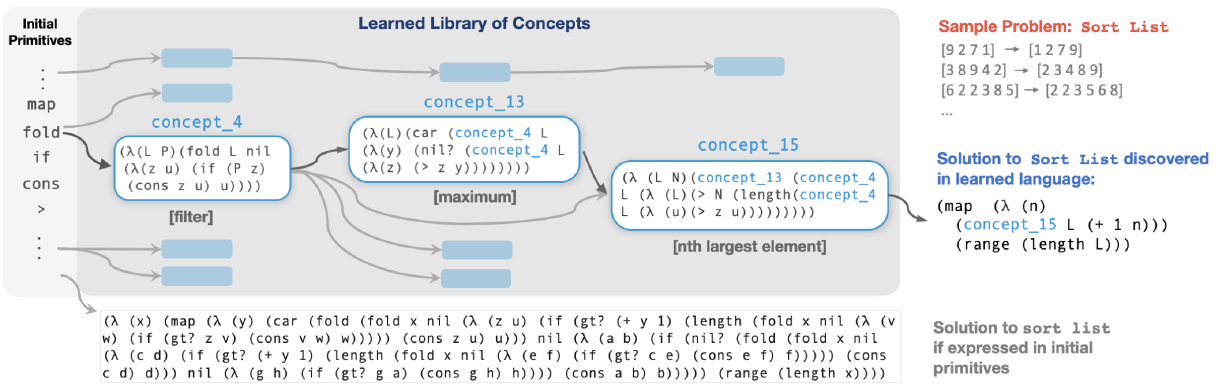
\includegraphics[width=\textwidth]{DreamCoderCompositionality.png}
    \end{figure}
\end{frame} 


% DreamCoder Slide 11: Applications of the Algorithm
\begin{frame}[c]{DreamCoder}{Applications}
    % Three columns of potential applications
    \begin{columns}[T]
        % First columns
        \begin{column}{0.33\textwidth}
            % List Processing
            \begin{figure}
                \centering
                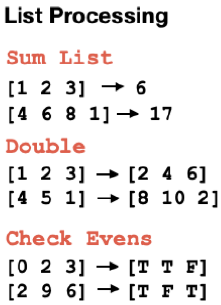
\includegraphics[height=0.35\textheight]{DreamCoderApp1.png}
            \end{figure}
            % Logo Graphics
            \begin{figure}
                \centering
                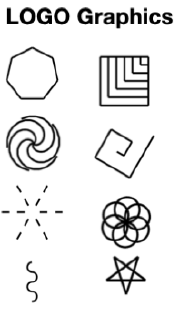
\includegraphics[height=0.35\textheight]{DreamCoderApp4.png}
            \end{figure}
        \end{column}
        % Second column
        \begin{column}{0.33\textwidth}
            % Block Towers
            \begin{figure}
                \centering
                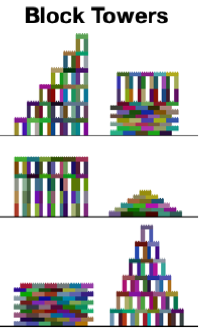
\includegraphics[height=0.35\textheight]{DreamCoderApp5.png}
            \end{figure}
            % Symbolic Regression
            \begin{figure}
                \centering
                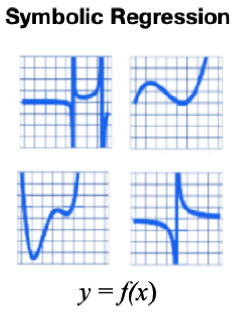
\includegraphics[height=0.35\textheight]{DreamCoderApp6.png}
            \end{figure}
        \end{column}
        % Third column
        \begin{column}{0.33\textwidth}
            % Recursive Programming
            \begin{figure}
                \centering
                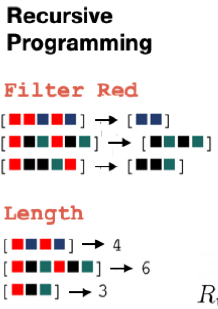
\includegraphics[height=0.35\textheight]{DreamCoderApp7.png}
            \end{figure}
            % Physical Laws
            \begin{figure}
                \centering
                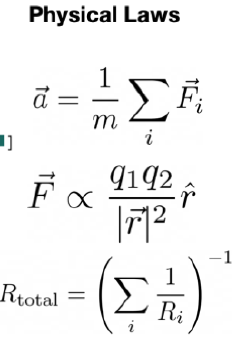
\includegraphics[height=0.35\textheight]{DreamCoderApp8.png}
            \end{figure}
        \end{column}
    \end{columns}
\end{frame}


% DreamCoder Slide 12: Applications of the Algorithm
\begin{frame}[c]{DreamCoder}{Applications}
    \centering
    \begin{figure}
        \centering
        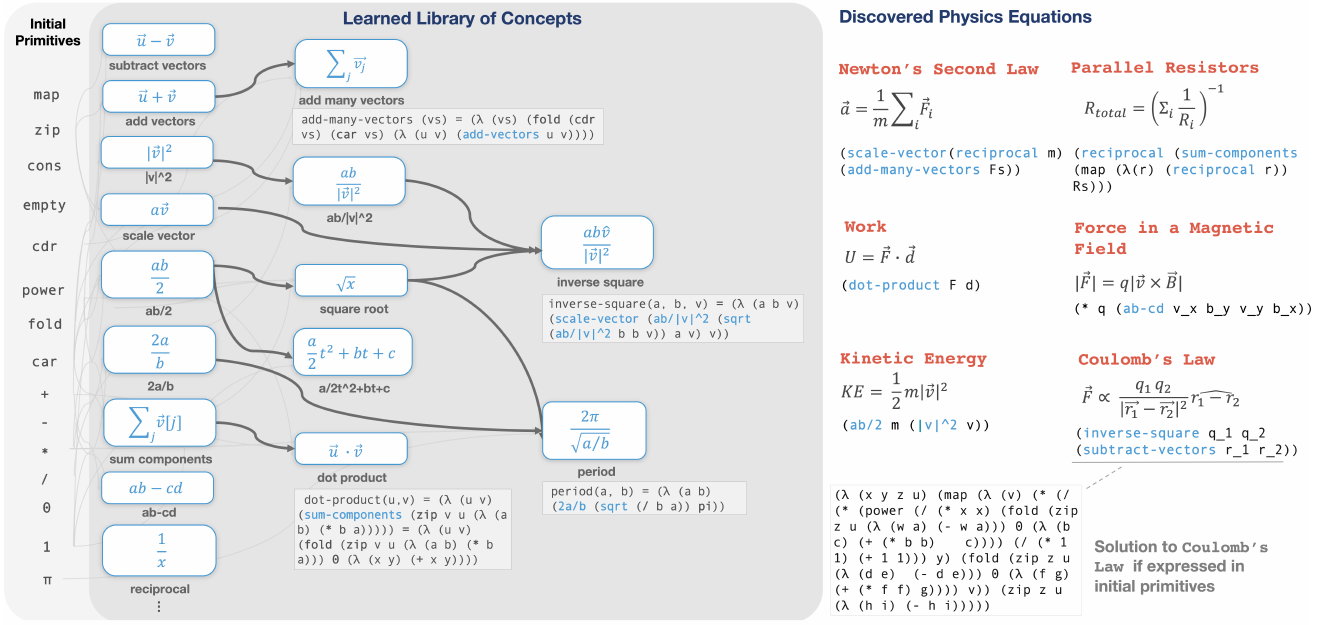
\includegraphics[width=0.95\textwidth]{DreamCoderApplication1.png}
        \caption{Learned library for physics equations.}
    \end{figure}
\end{frame}


% DreamCoder Slide 13: Applications of the Algorithm
\begin{frame}[c]{DreamCoder}{Applications}
    \centering
    \begin{figure}
        \centering
        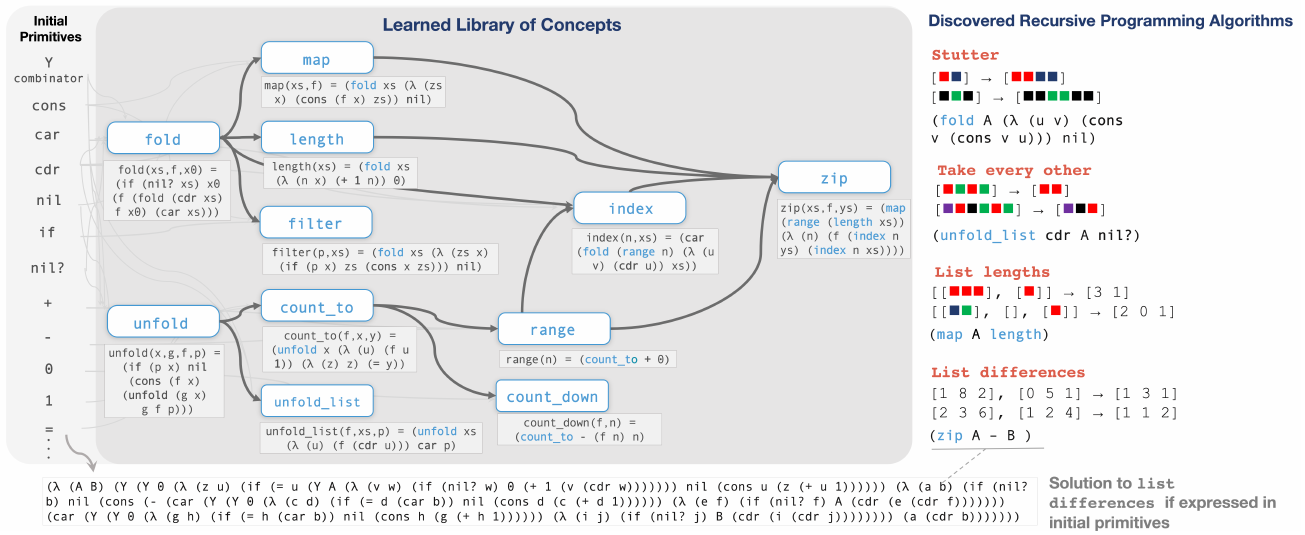
\includegraphics[width=0.95\textwidth]{DreamCoderApplication2.png}
        \caption{Learned library for recursive programming algorithm.}
    \end{figure}
\end{frame}


% DreamCoder Slide 14: Applications of the Algorithm
\begin{frame}[c]{DreamCoder}{Applications}
    \centering
    \begin{figure}
        \centering
        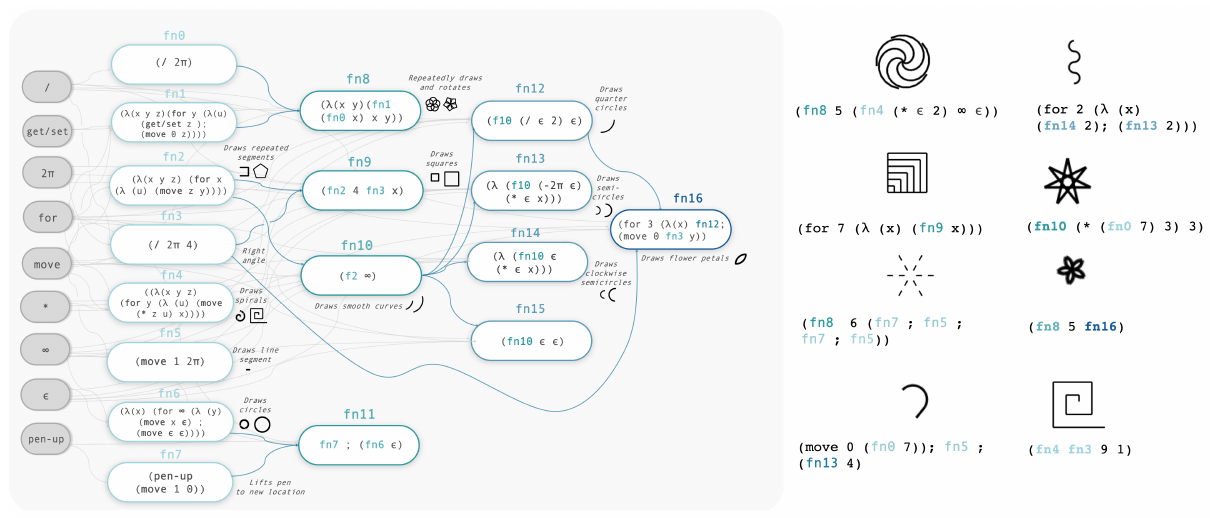
\includegraphics[width=\textwidth]{DreamCoderApplication3.png}
        \caption{Learned library for LOGO graphics.}
    \end{figure}
\end{frame}


% DreamCoder Slide 15: Applications of the Algorithm
\begin{frame}[c]{DreamCoder}{Applications}
    \centering
    \begin{figure}
        \centering
        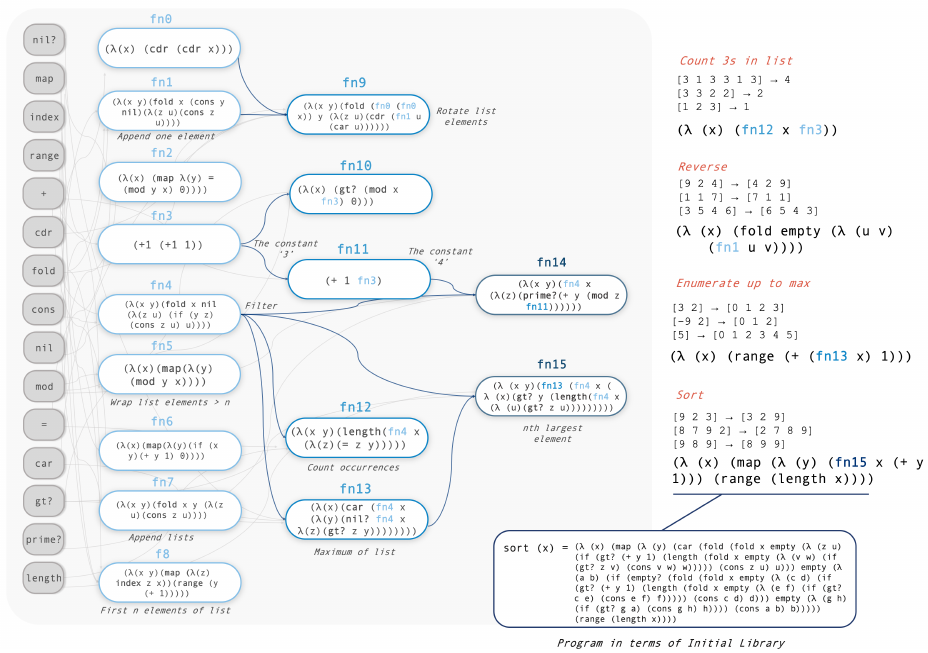
\includegraphics[width=0.65\textwidth]{DreamCoderApplication4.png}
        \caption{Learned library for list processing.}
    \end{figure}
\end{frame}


% DreamCoer Slide 16: Summary
\begin{frame}[c]{DreamCoder}{Take-Aways}
    \centering
    \begin{itemize}
        \item Combining probabilistic programming with a DSL-learning procedure and novel probabilistic inference procedure
              to iteratively learn to represent a problem's domain allows one to gain the ability to solve a problem
        \item Such applications require highly complex codebase structures across multiple languages
        \item For more complex examples reliant on a highly efficient inference procedure
    \end{itemize}
\end{frame}




% Why Do We even Need Probabilistic Programming? (5-10 slides)
\section{Why Do We even Need Probabilistic Programming?}





% Underlying Theoretical Ideas (60+ slides)
\section{Underlying Theoretical Ideas}




% Different Types of Probabilistic Programming Systems (~20 slides)
\section{Different Types of Probabilistic Programming Systems}







%
%\AERbeamerSetFooterText{References}%
%\begin{frame}[allowframebreaks]{References}%
%    \printbibliography[heading=none]%
%\end{frame}%
%
% End with titlepage
%\AERbeamerTitlePageDefault%
%
%
\end{document}%
%
%
